\section{Degree distribution}

\subsection*{Purpose}

\paragraph{}
To compare the vertex degree distribution of the original graph stream and the graph depicted by the summarized sketch.

\subsection*{Results}

\begin{figure}[H]
    \centering 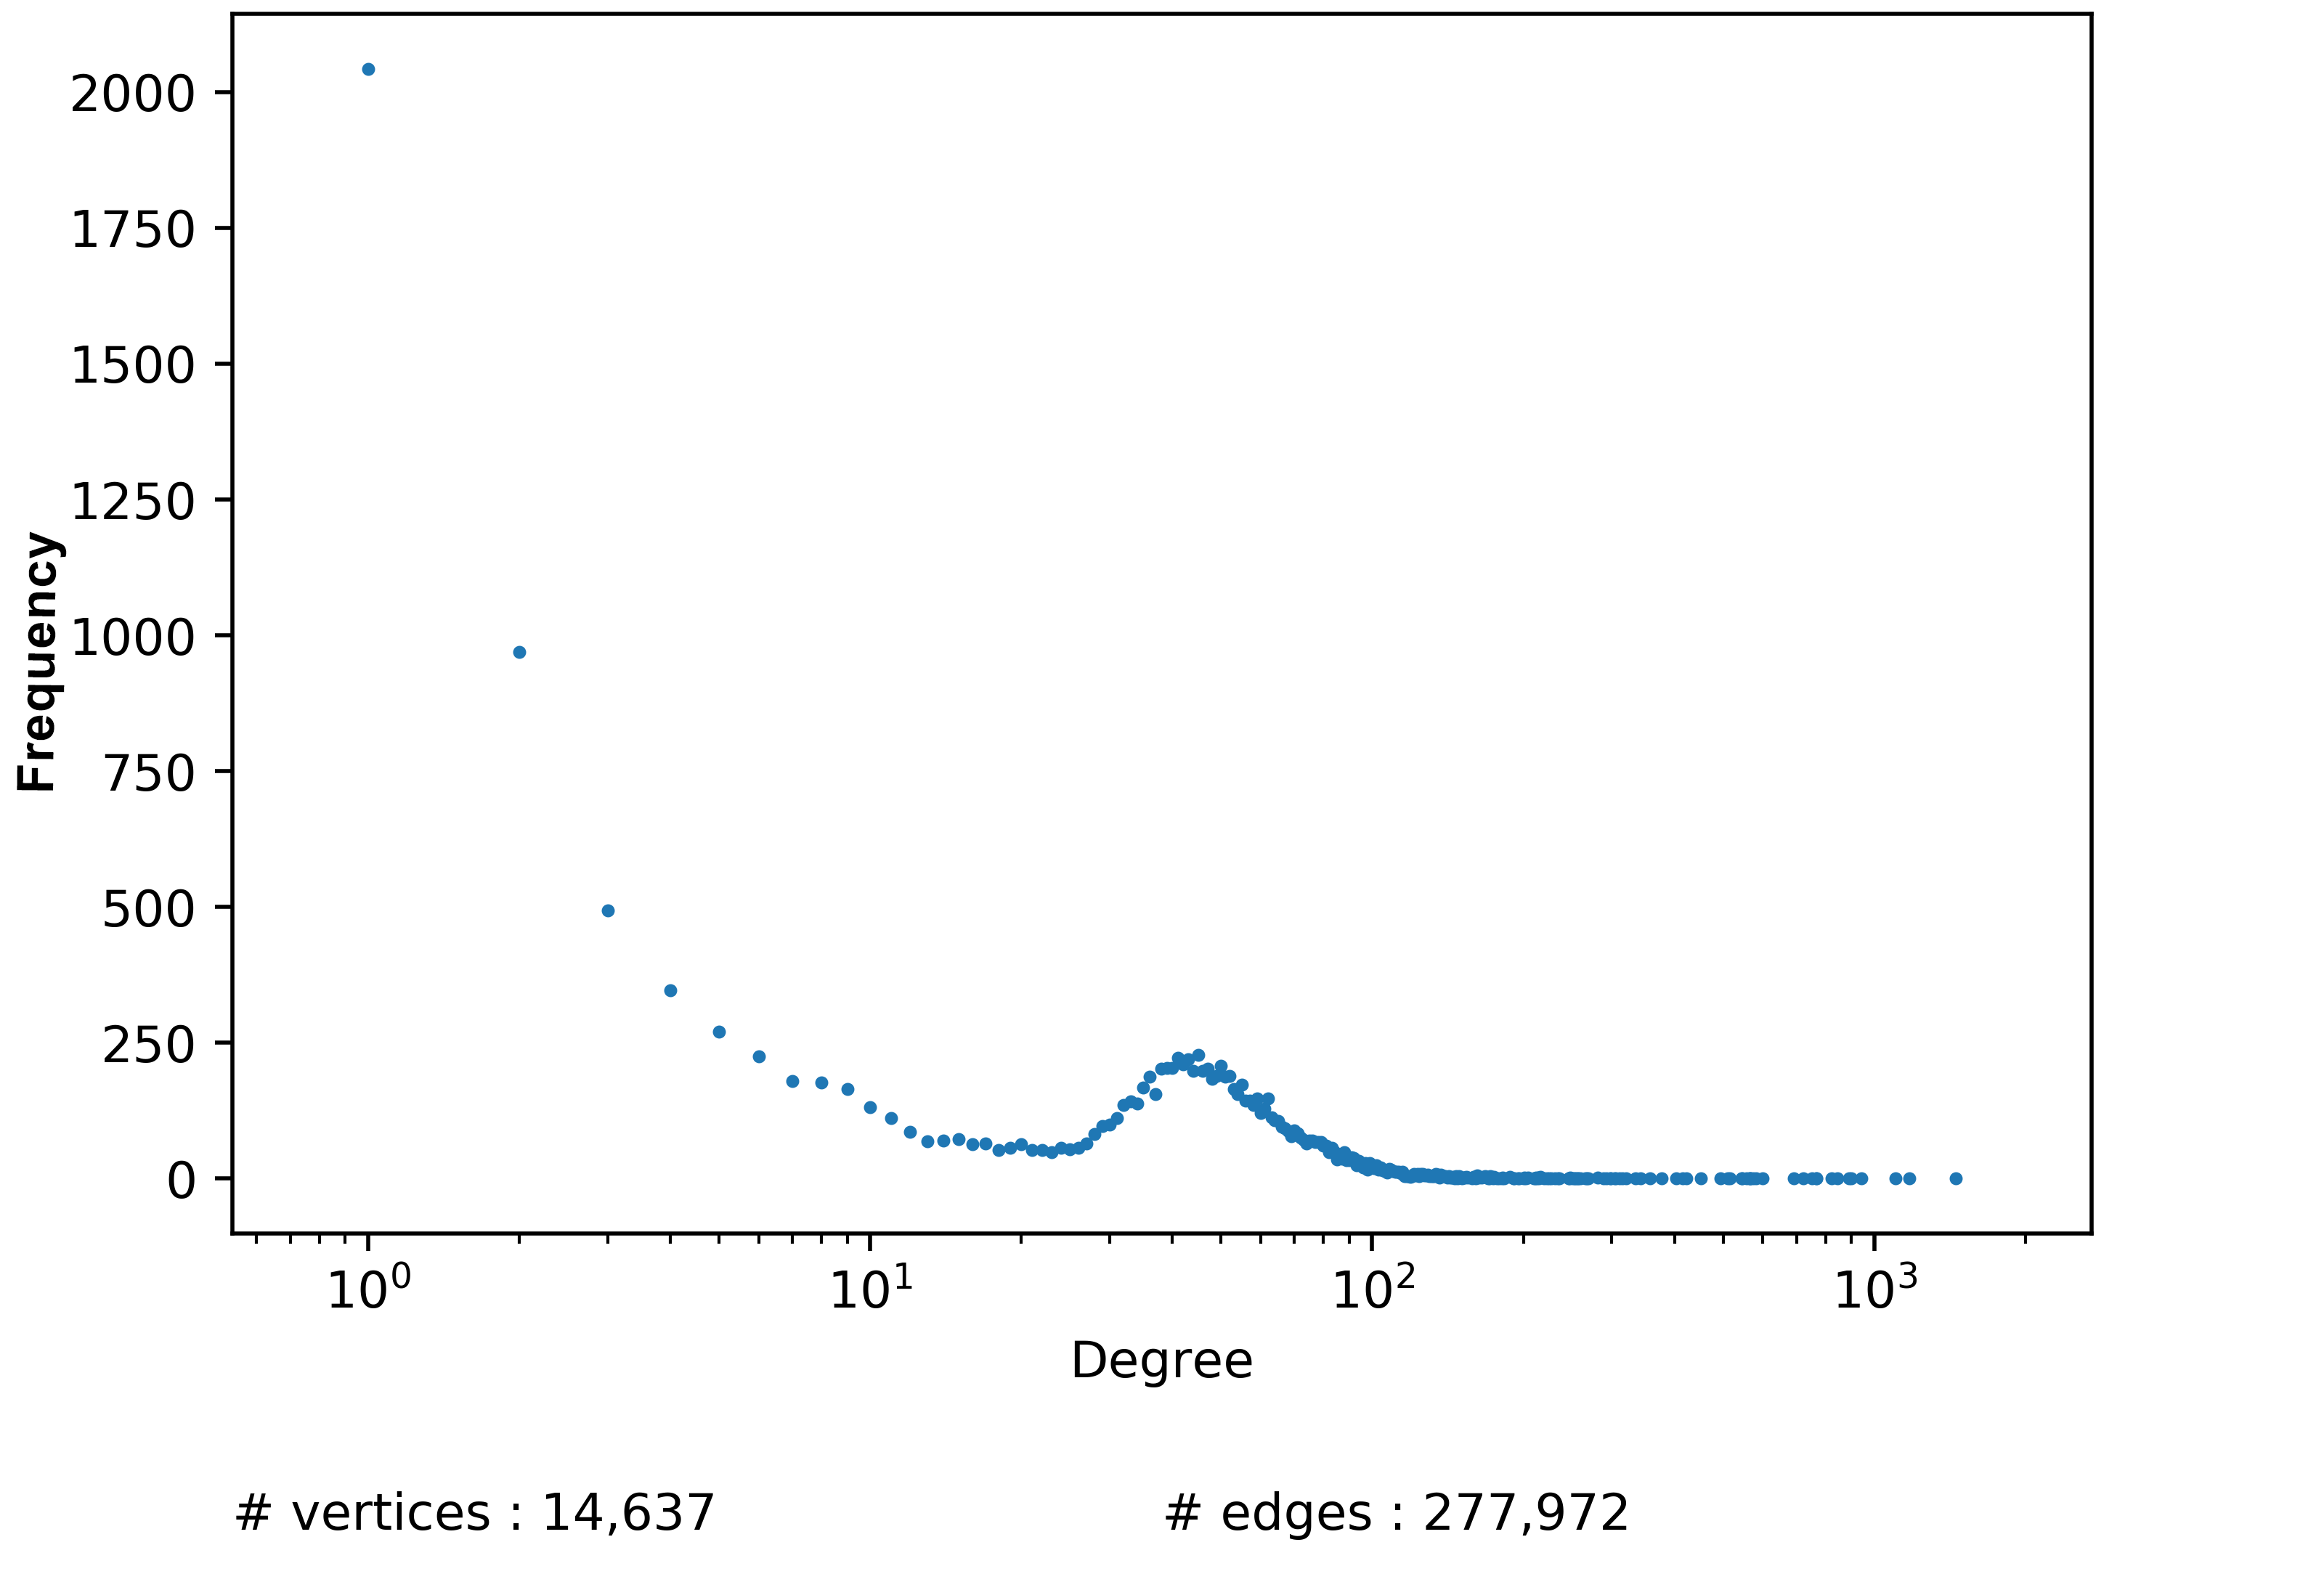
\includegraphics[width=0.85\textwidth]{results/dd/unicorn-wget-dd-fullgraph}
    \vspace{-0.5cm}
    \caption{Degree distribution of FullGraph for unicorn-wget dataset}
    \label{fig:unicorn-wget-dd-fullgraph}
\end{figure}

\begin{figure}[H]
    \centering 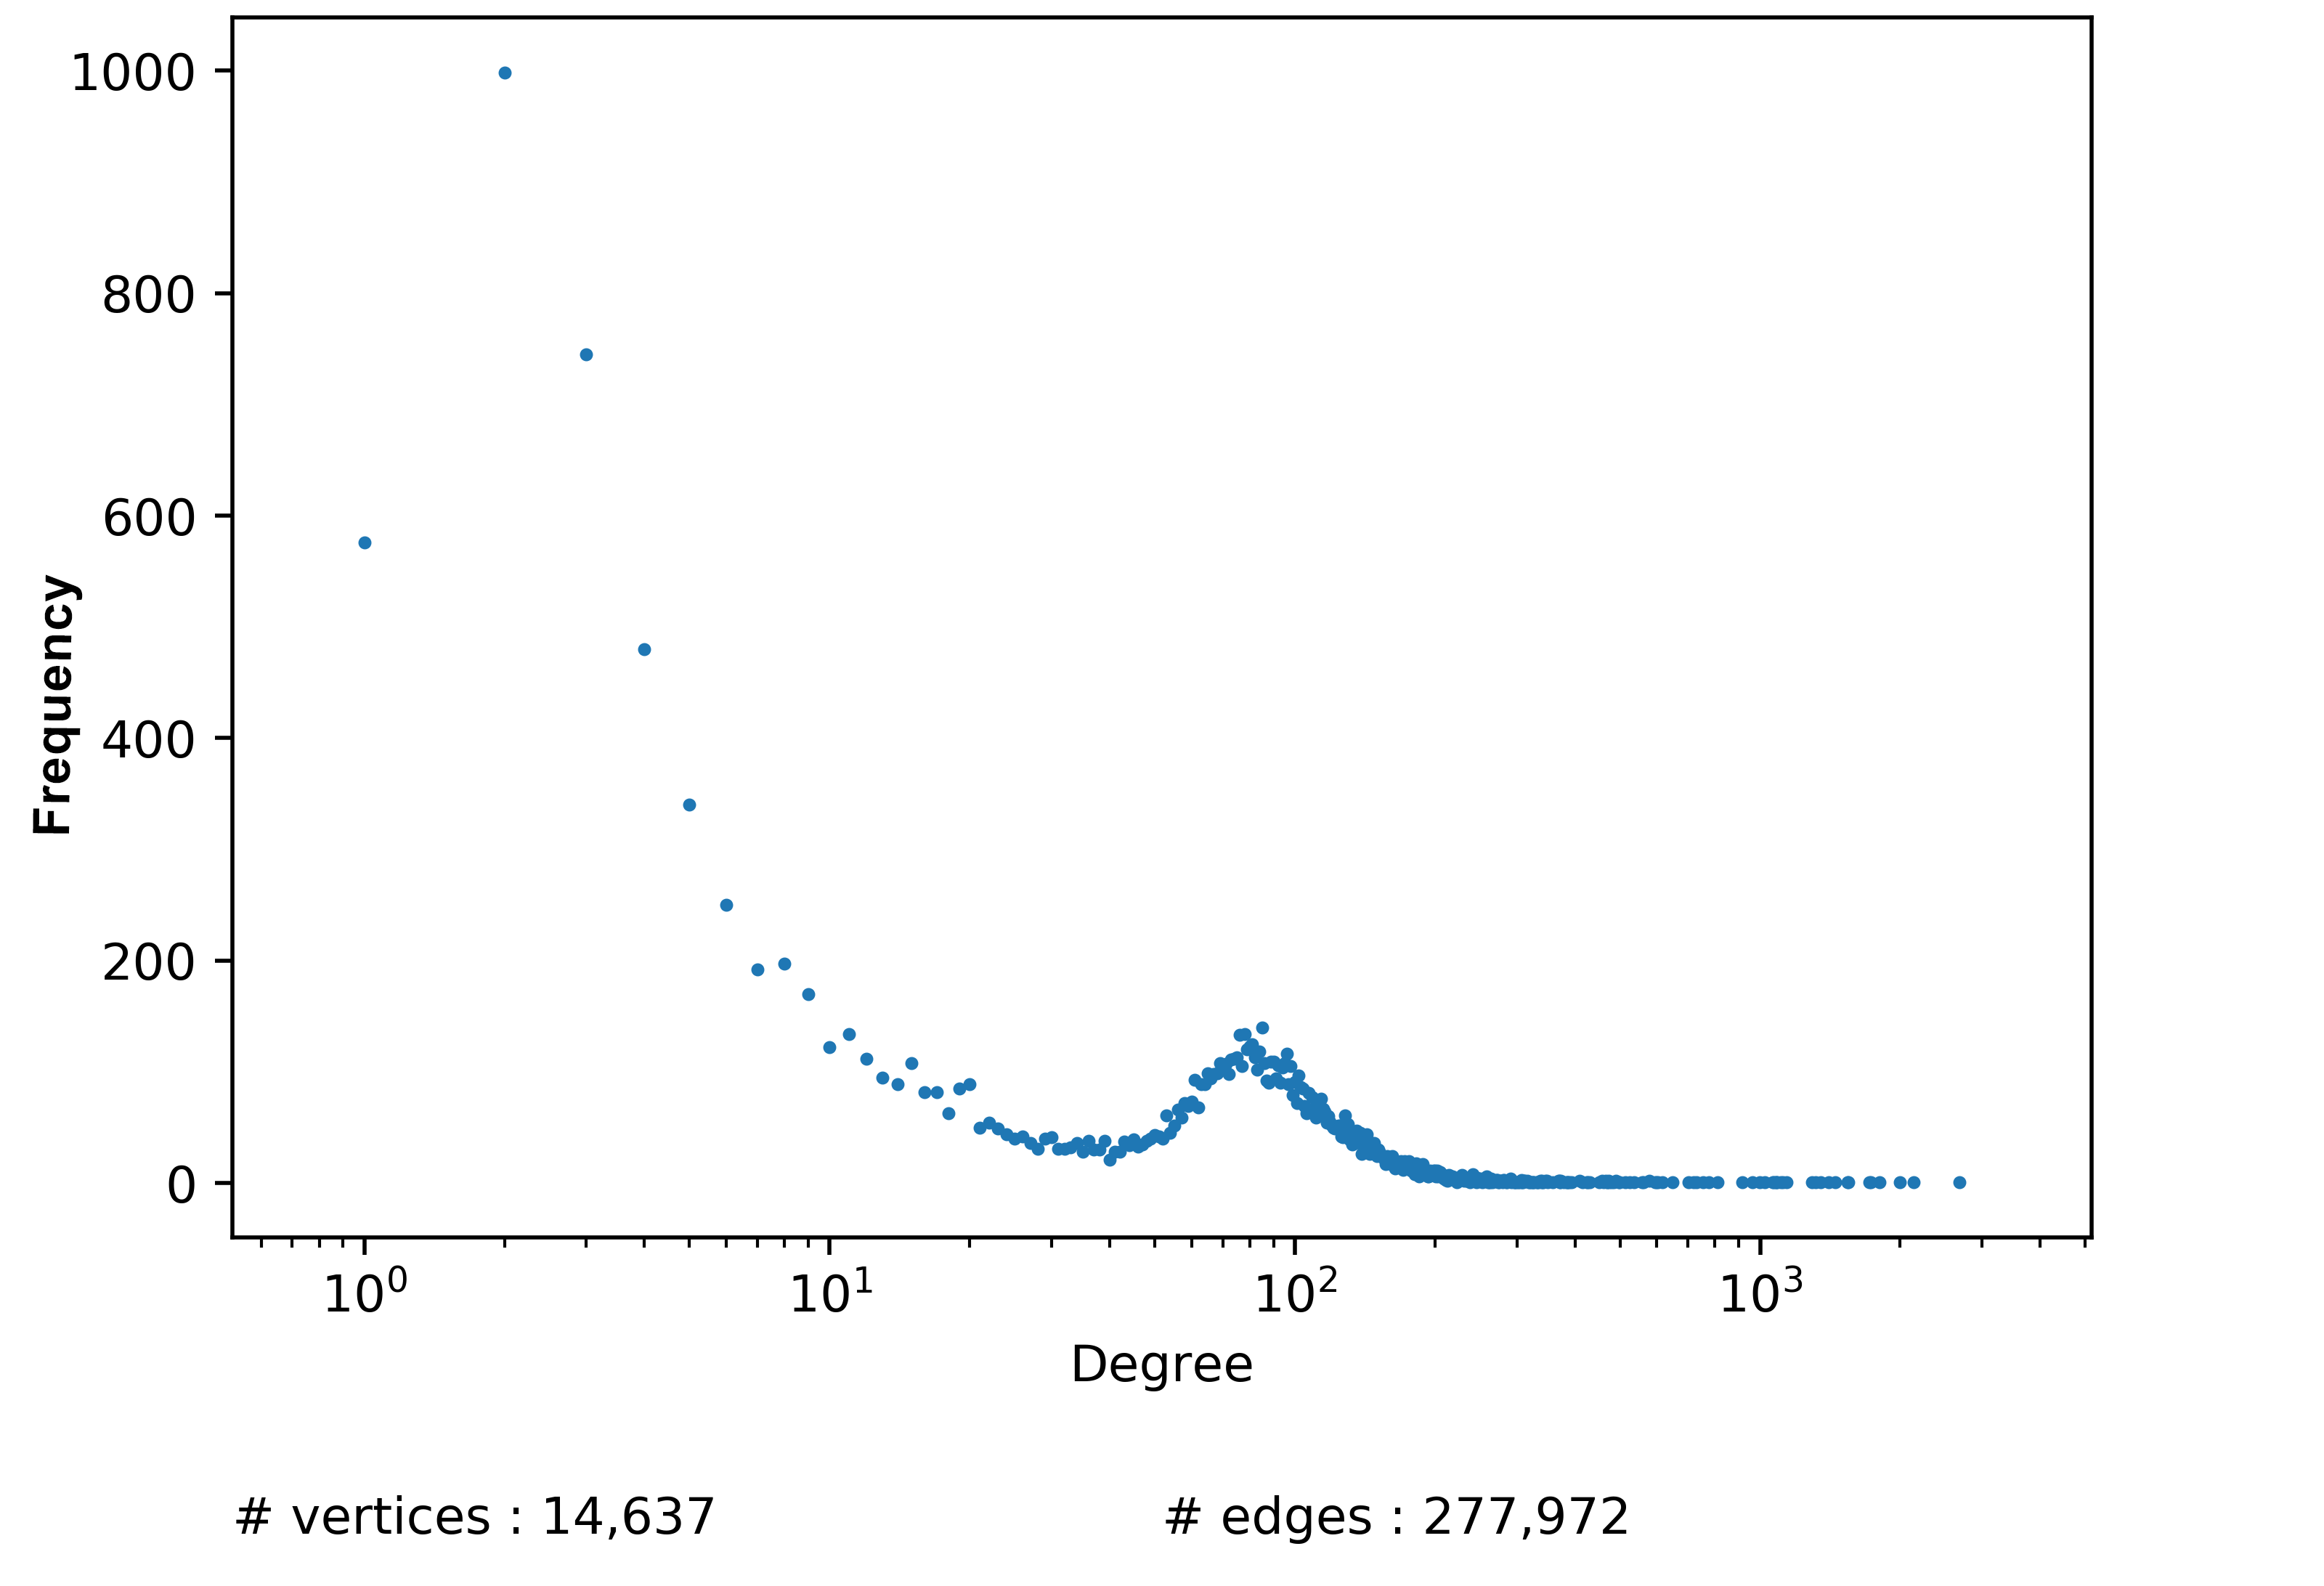
\includegraphics[width=0.85\textwidth]{results/dd/unicorn-wget-dd-countmin_1024}
    \vspace{-0.5cm}
    \caption{Degree distribution of CountMin for unicorn-wget dataset}
    \label{fig:unicorn-wget-dd-countmin_1024}
\end{figure}

\begin{figure}[H]
    \centering 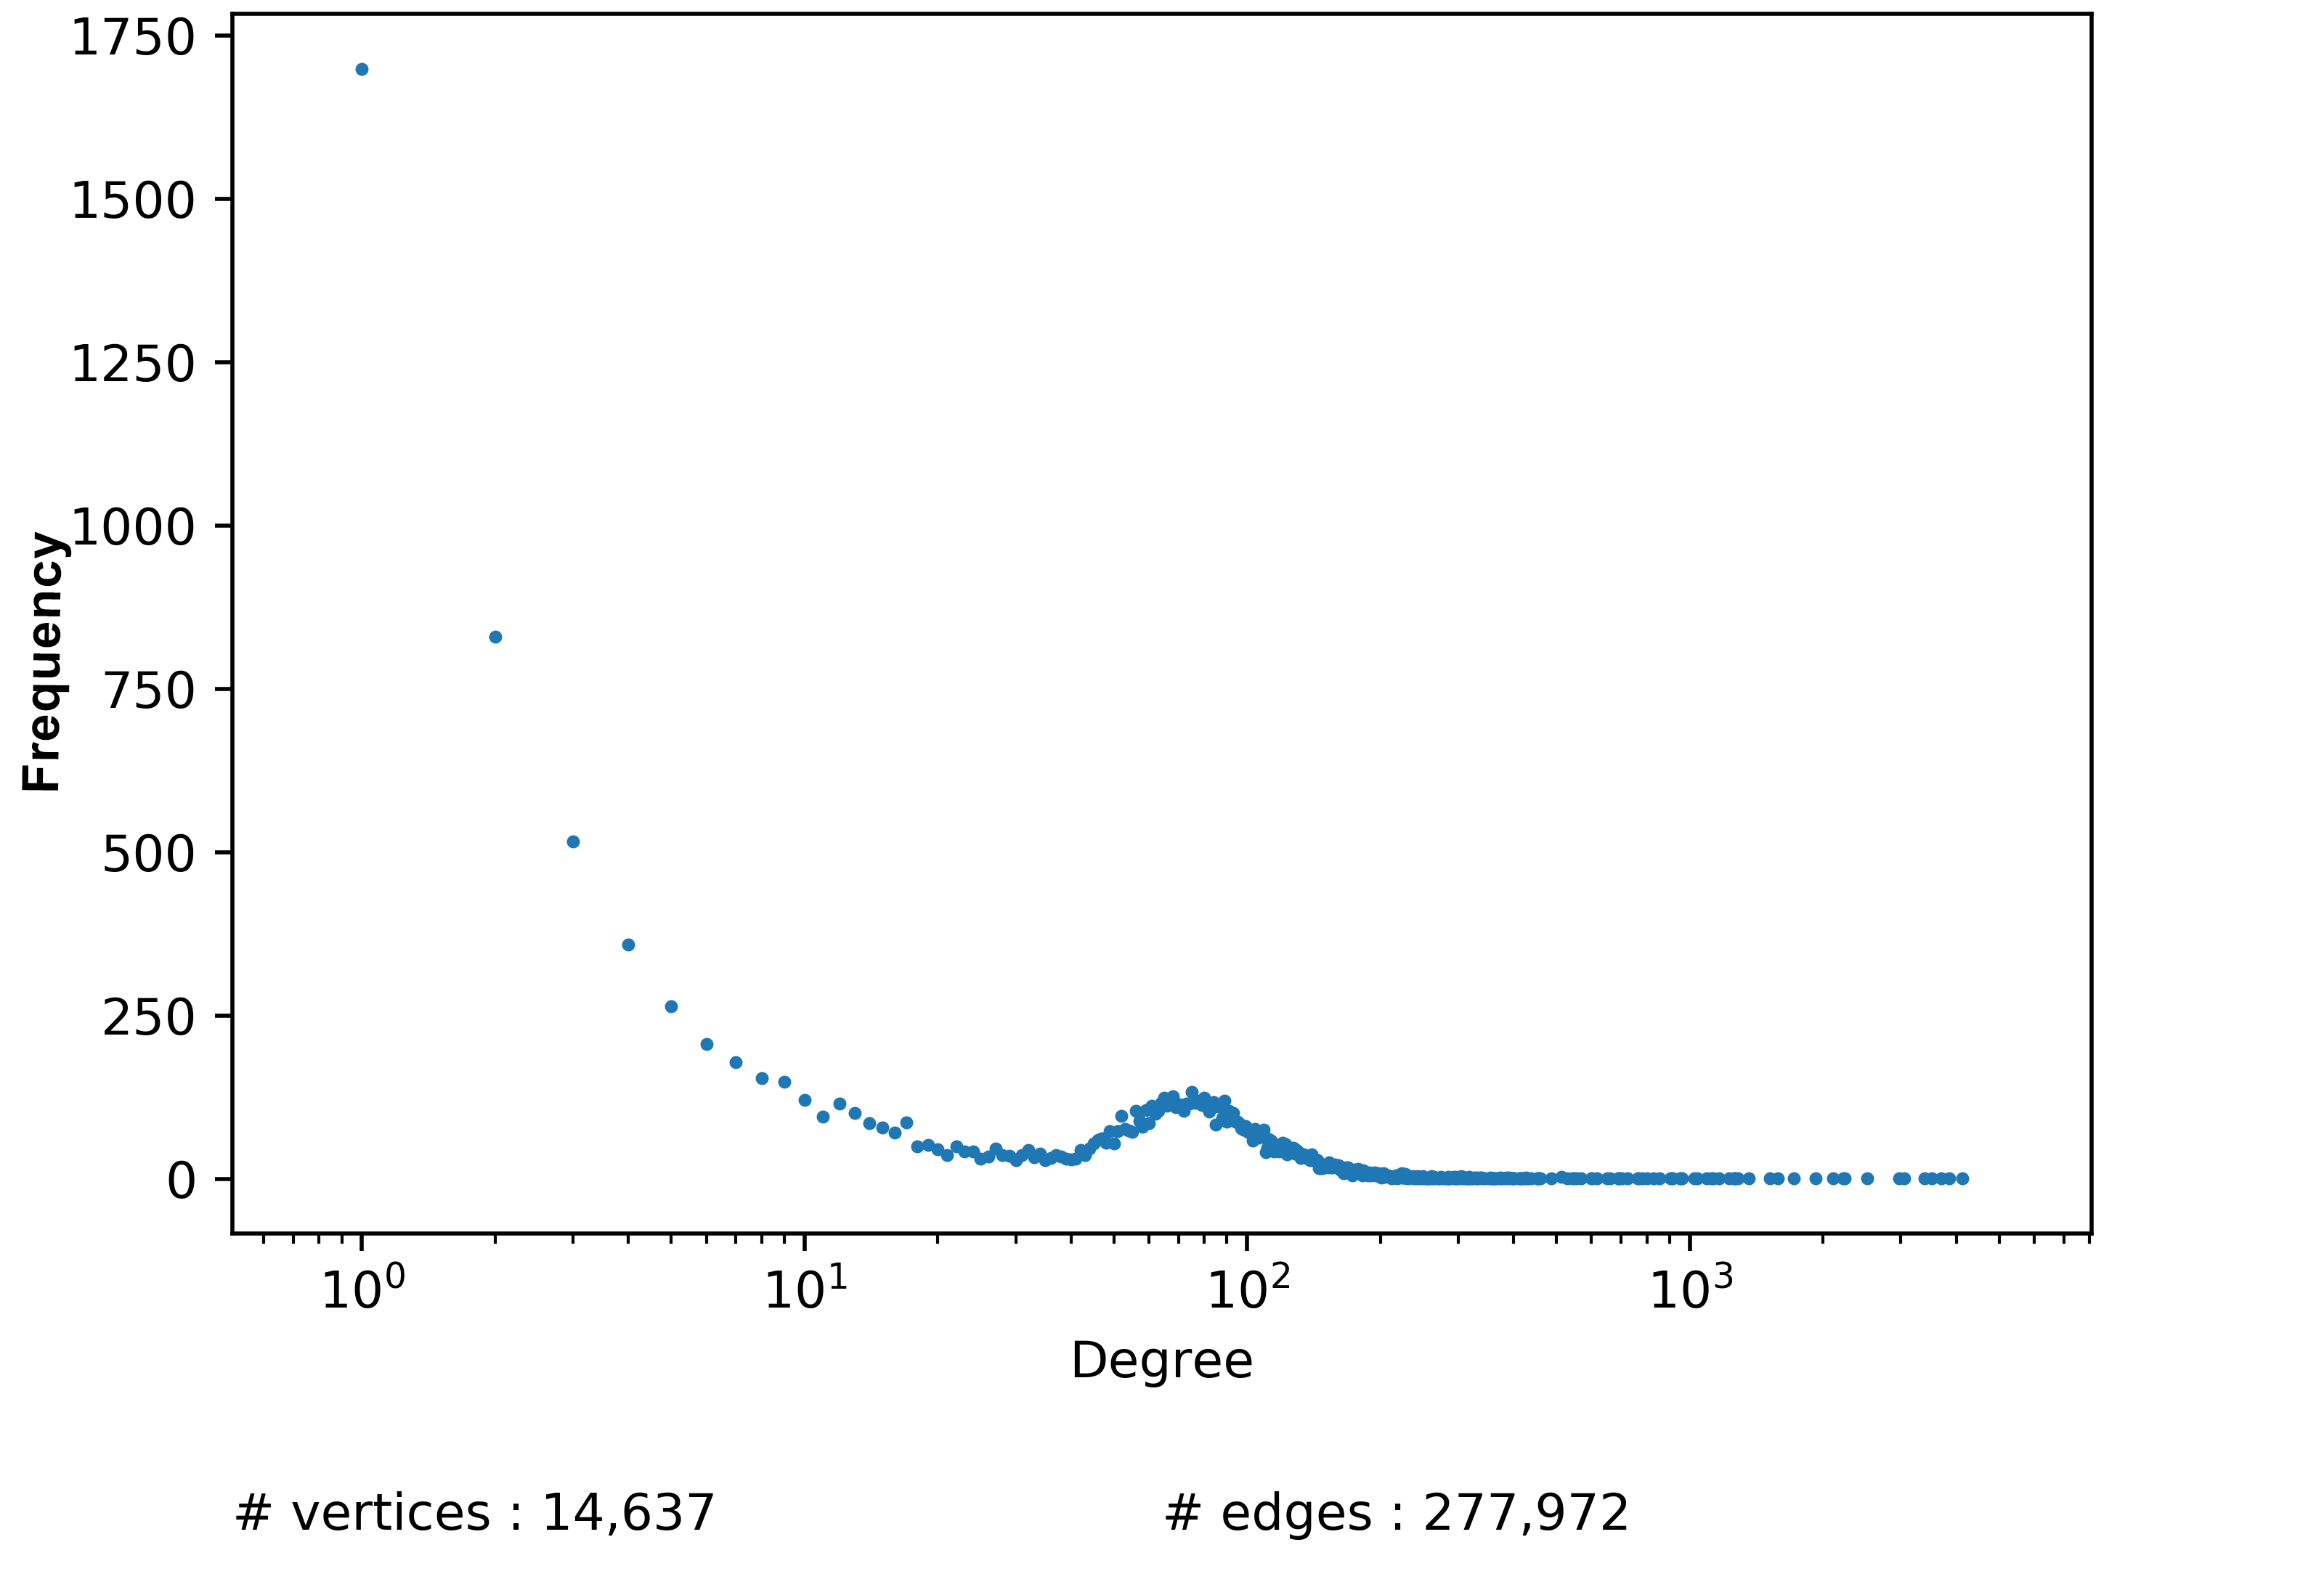
\includegraphics[width=0.85\textwidth]{results/dd/unicorn-wget-dd-gsketch_1024}
    \vspace{-0.5cm}
    \caption{Degree distribution of gSketch for unicorn-wget dataset}
    \label{fig:unicorn-wget-dd-gsketch_1024}
\end{figure}

\begin{figure}[H]
    \centering 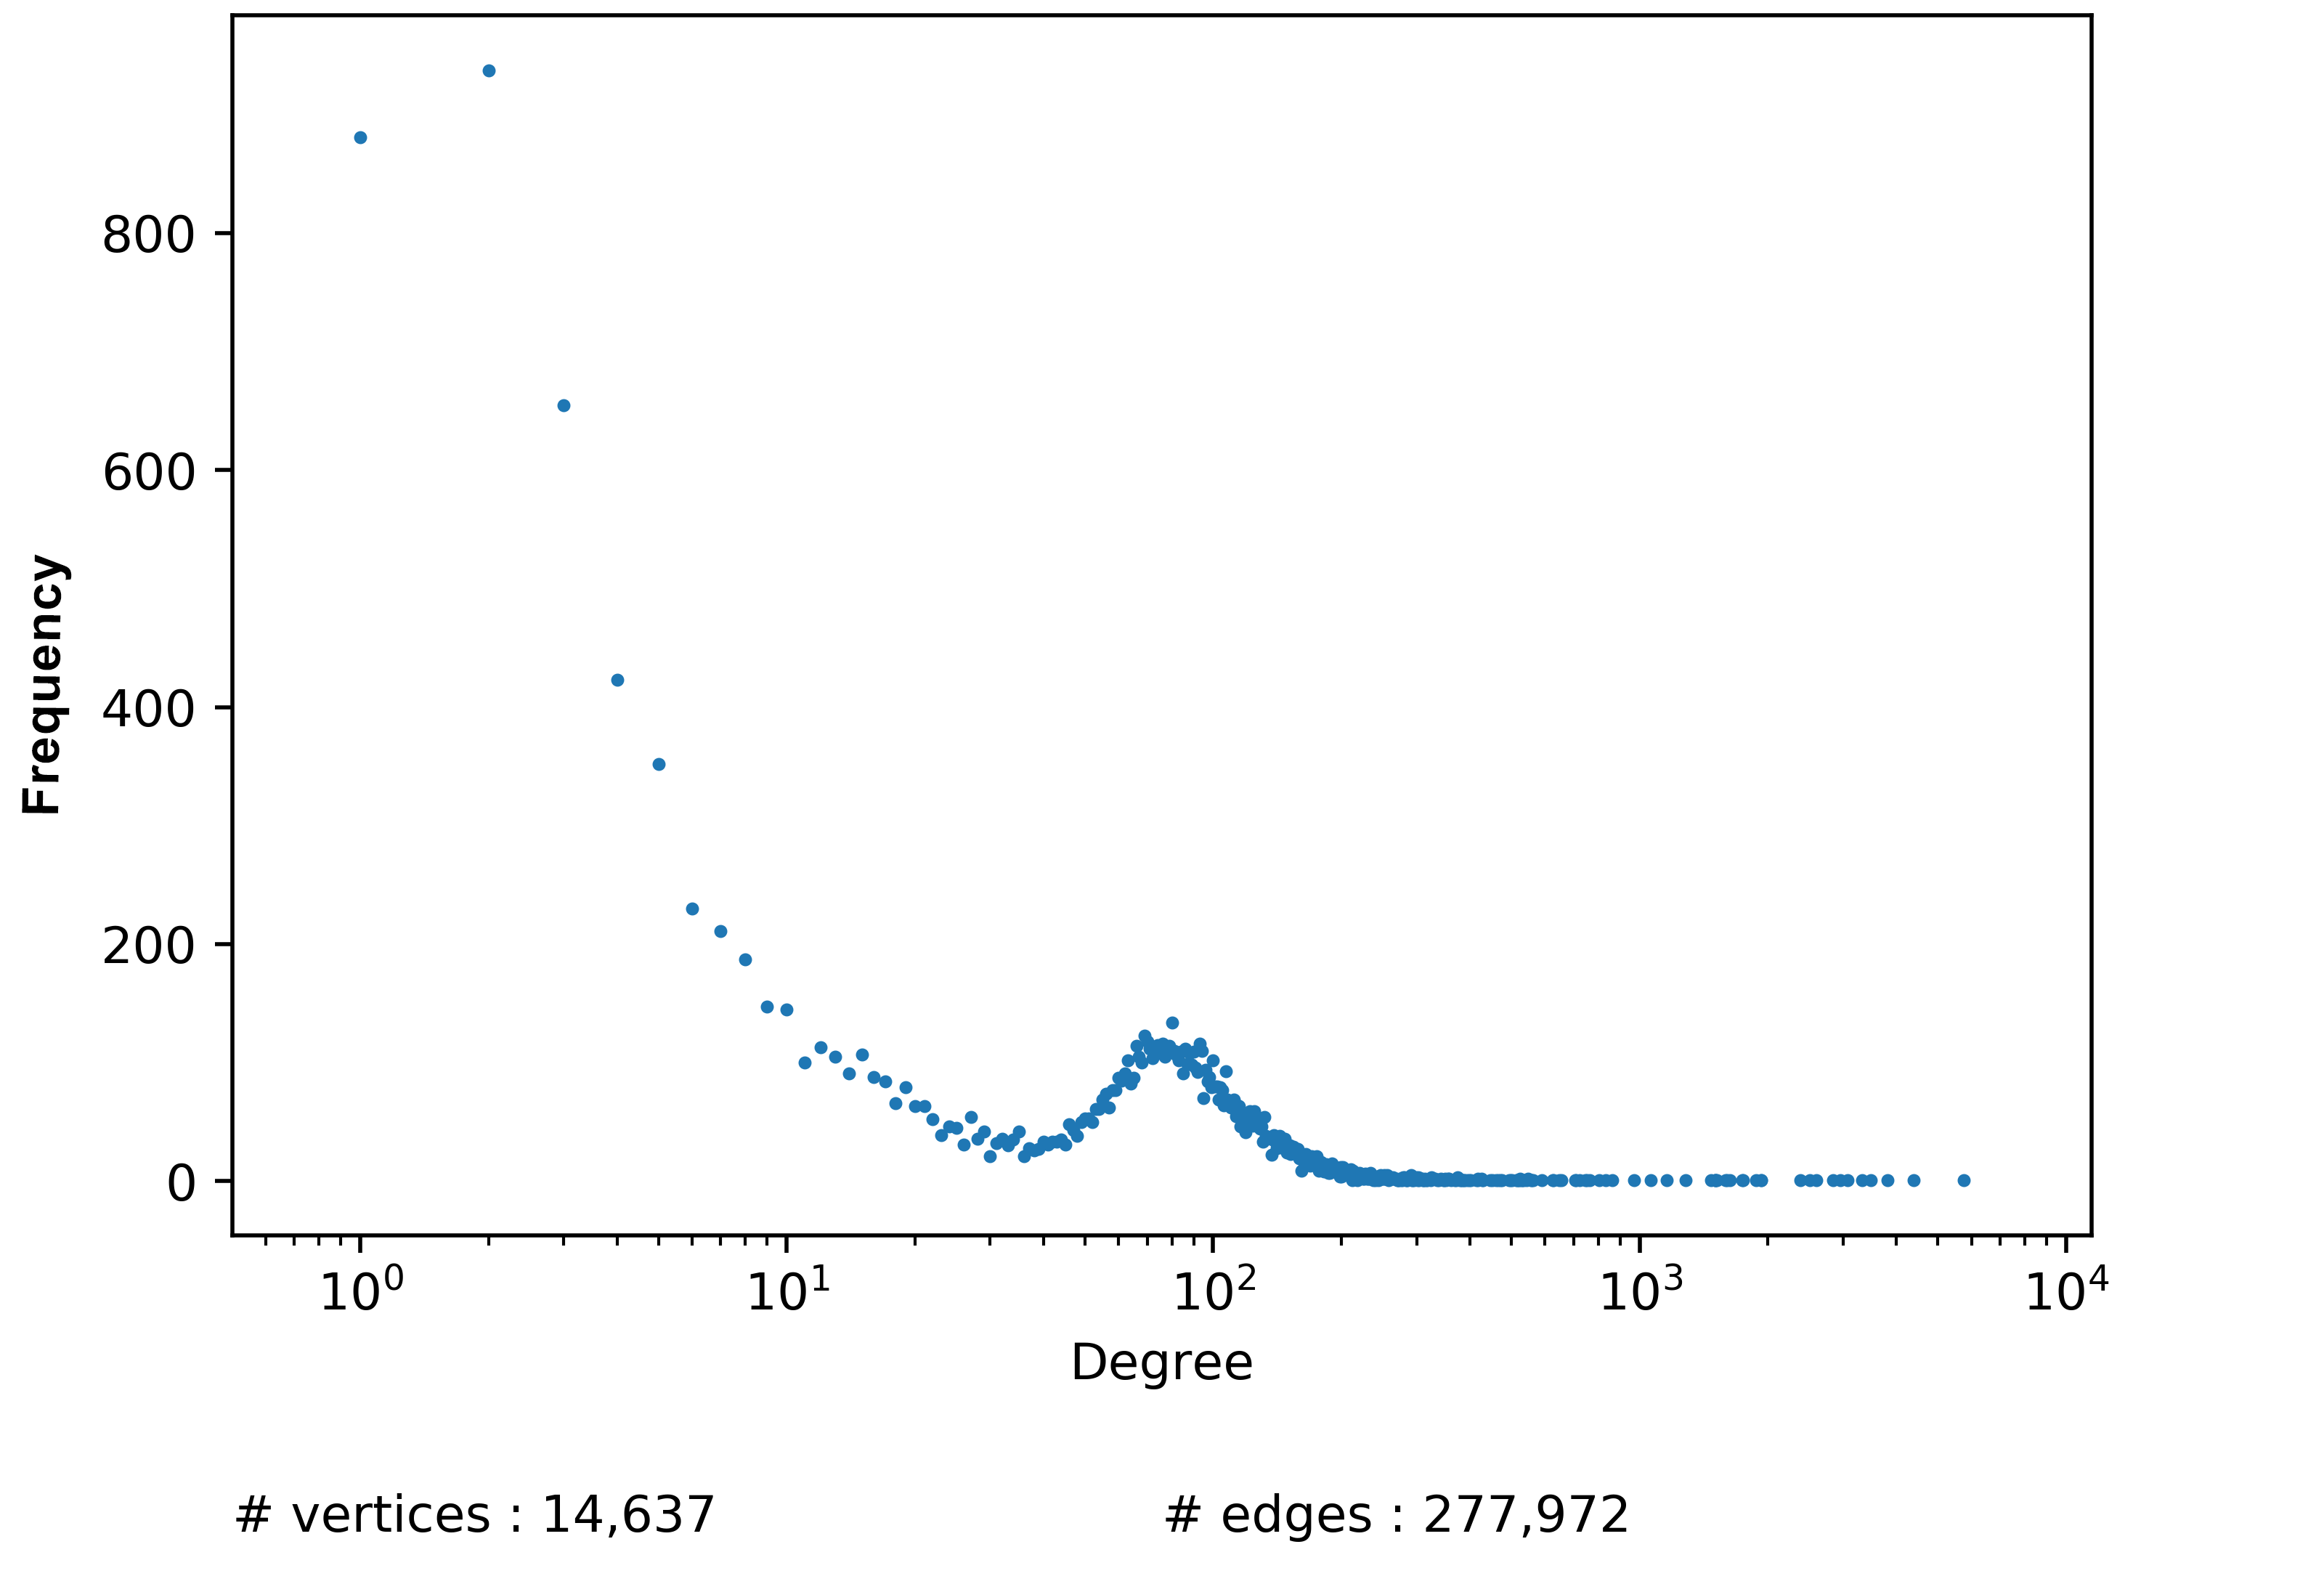
\includegraphics[width=0.85\textwidth]{results/dd/unicorn-wget-dd-tcm_1024}
    \vspace{-0.5cm}
    \caption{Degree distribution of TCM for unicorn-wget dataset}
    \label{fig:unicorn-wget-dd-tcm_1024}
\end{figure}

\begin{figure}[H]
    \centering 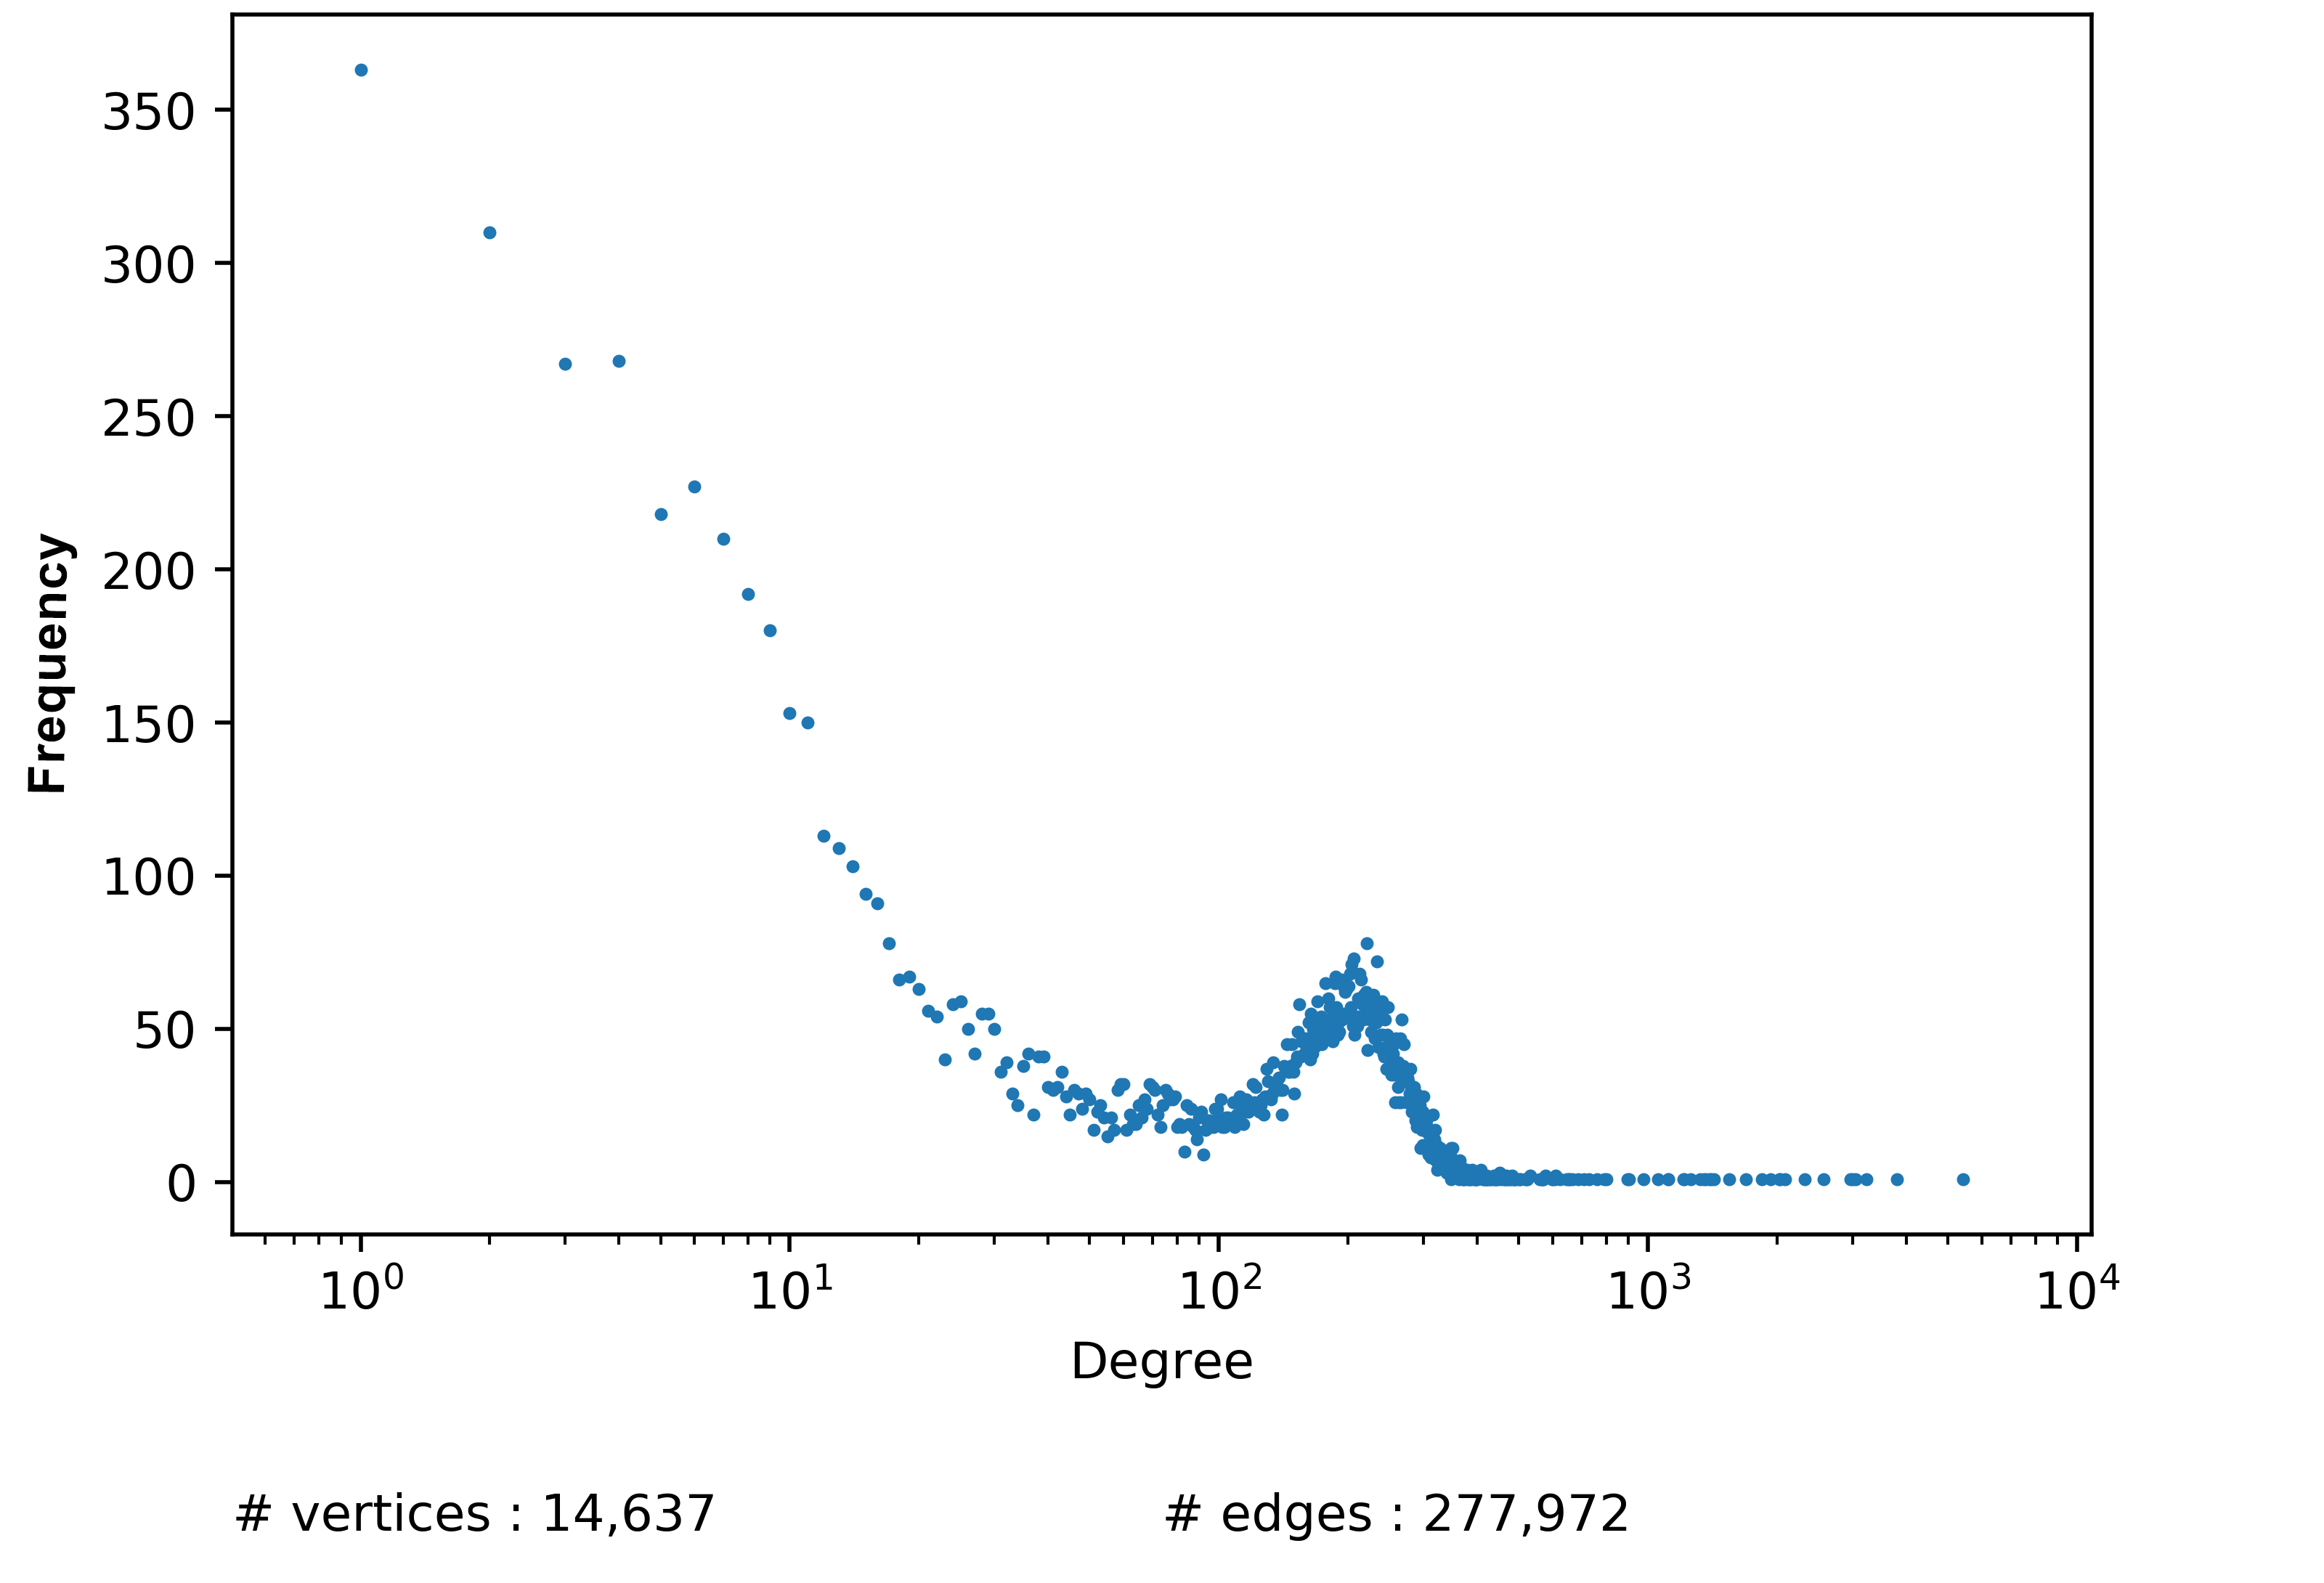
\includegraphics[width=0.85\textwidth]{results/dd/unicorn-wget-dd-gmatrix_1024}
    \vspace{-0.5cm}
    \caption{Degree distribution of GMatrix for unicorn-wget dataset}
    \label{fig:unicorn-wget-dd-gmatrix_1024}
\end{figure}

\begin{figure}[H]
    \centering 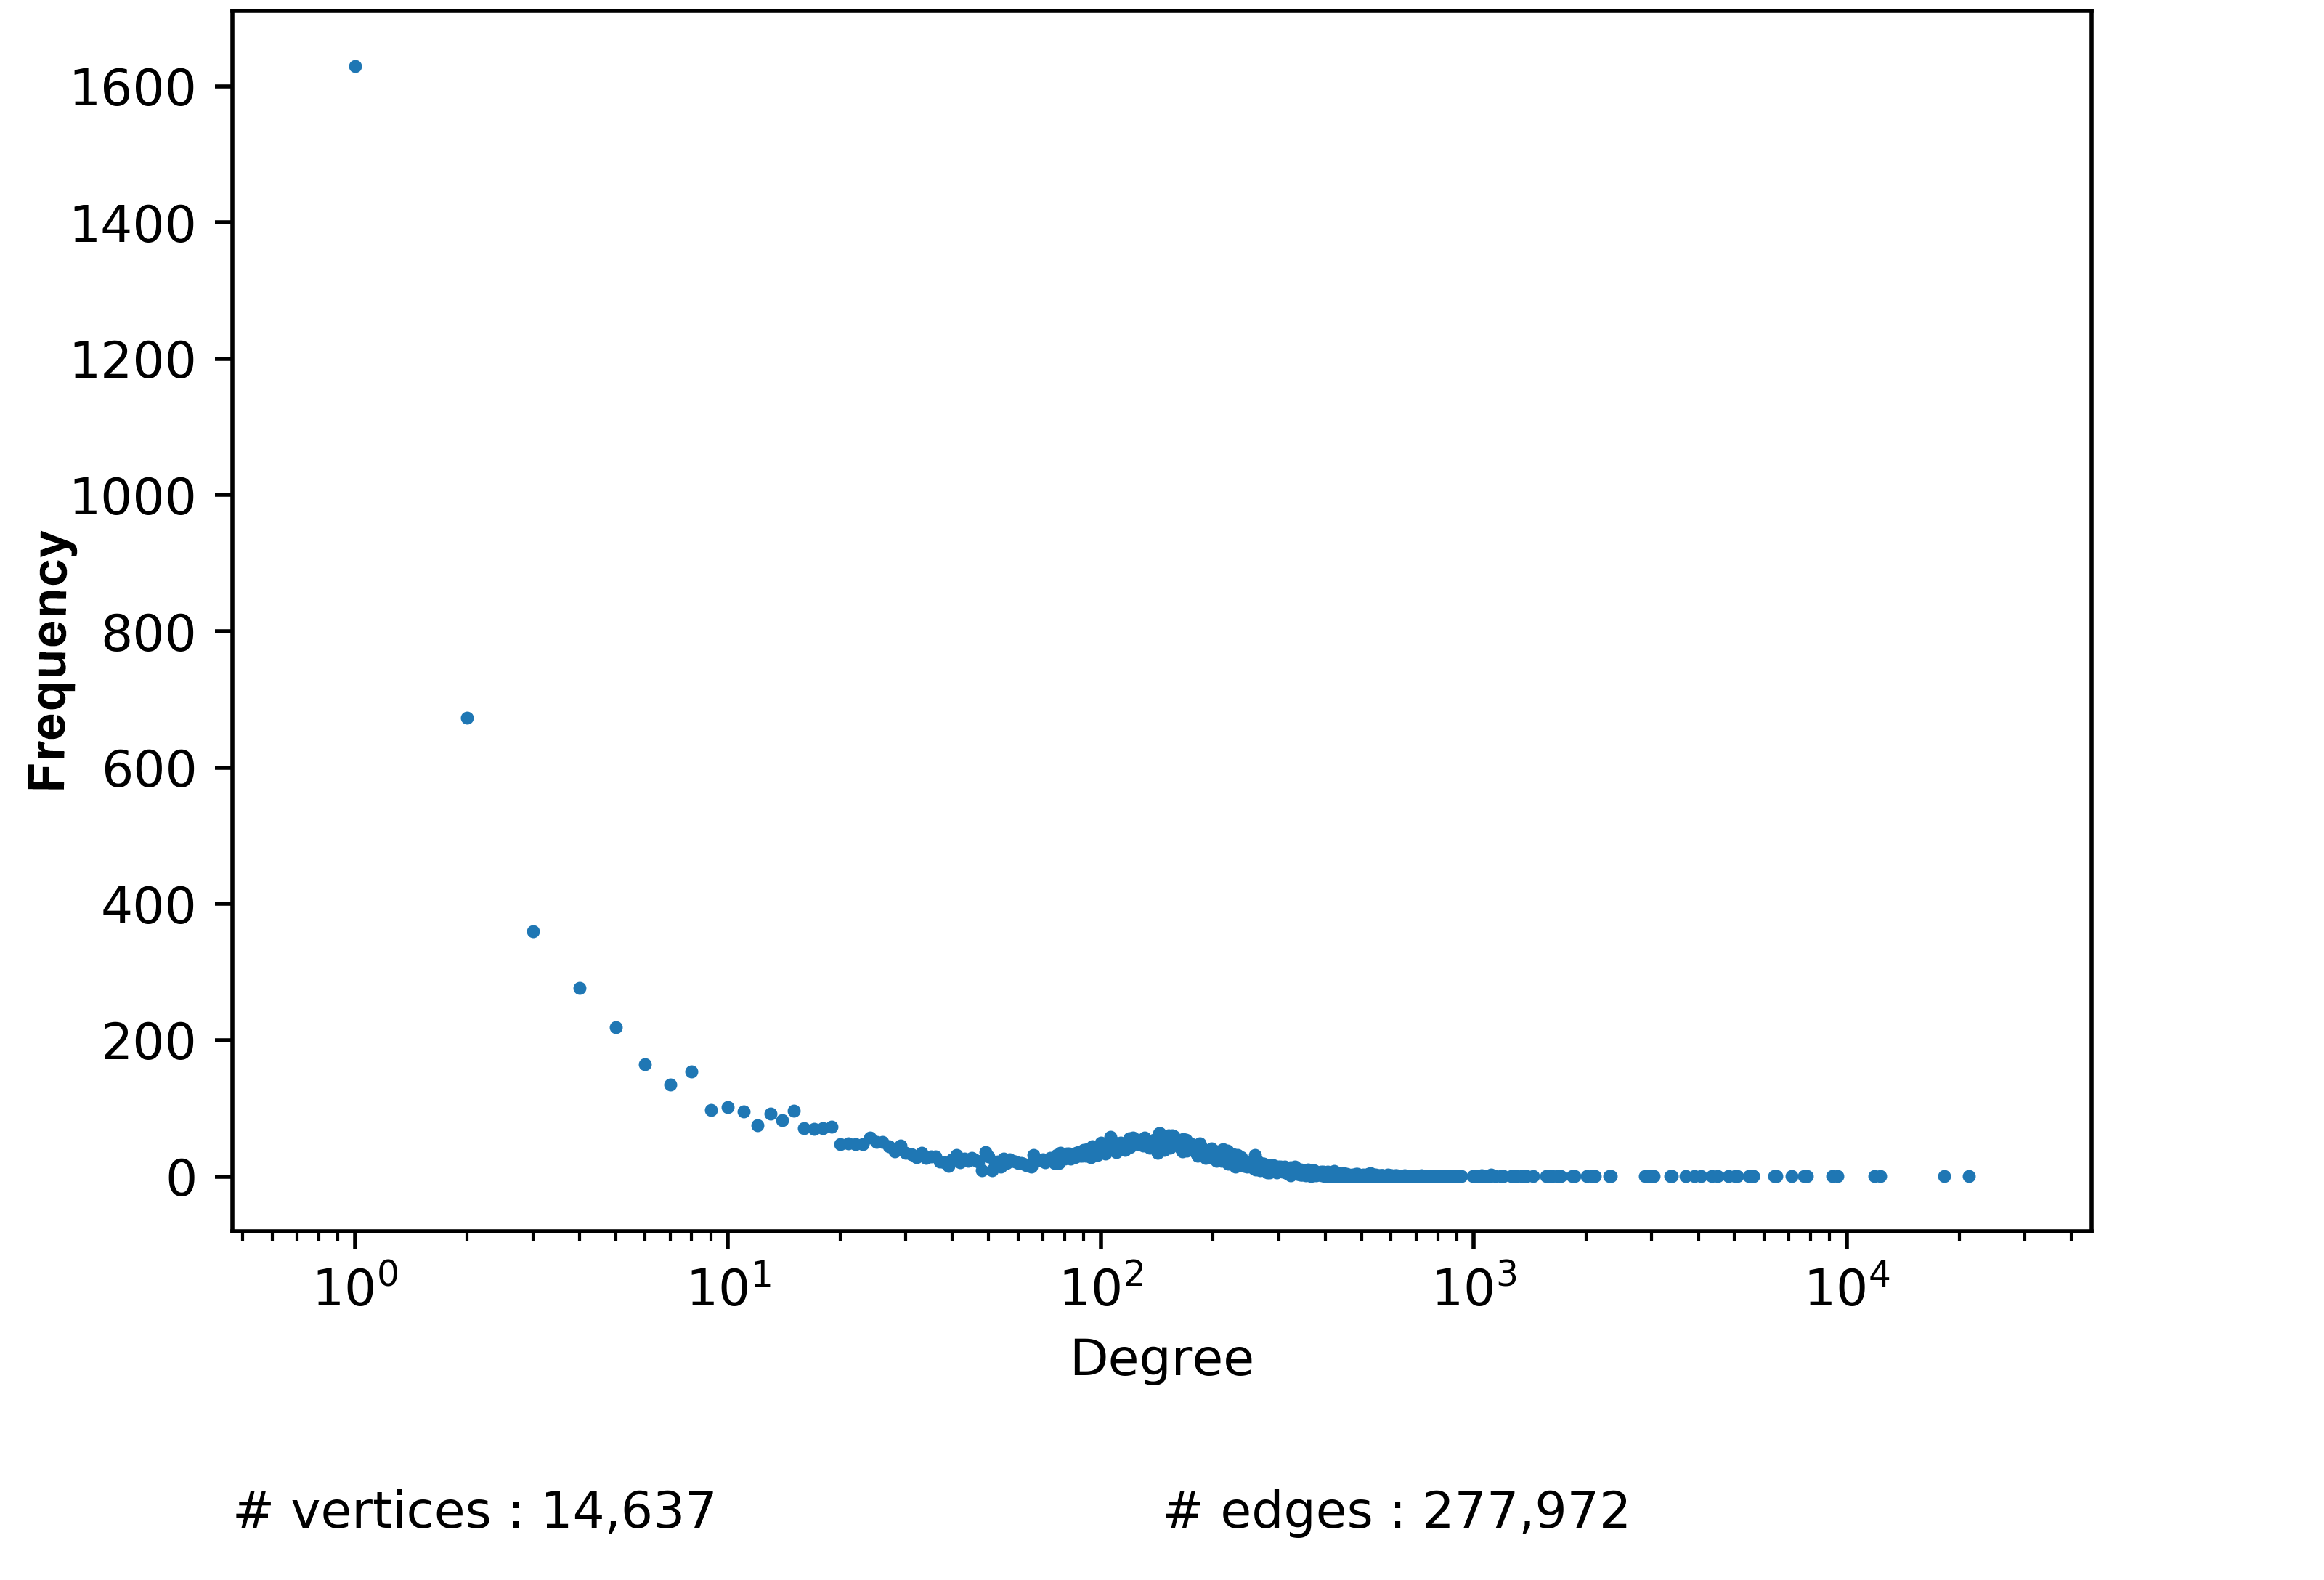
\includegraphics[width=0.85\textwidth]{results/dd/unicorn-wget-dd-alpha_1024}
    \vspace{-0.5cm}
    \caption{Degree distribution of Alpha for unicorn-wget dataset}
    \label{fig:unicorn-wget-dd-alpha_1024}
\end{figure}

\subsection*{Observations and inferences}

\paragraph{}
The graphs depicted by the summarized sketches in \autoref{fig:unicorn-wget-dd-countmin_1024}, \autoref{fig:unicorn-wget-dd-gsketch_1024}, \autoref{fig:unicorn-wget-dd-tcm_1024}, \autoref{fig:unicorn-wget-dd-gmatrix_1024} and \autoref{fig:unicorn-wget-dd-alpha_1024} have the same shape of the degree distribution as that of the original graph depicted in \autoref{fig:unicorn-wget-dd-fullgraph}. Thus all the sketches have preserved the degree distribution property of the original graph to a certain extent.